\documentclass[a4paper, 11pt, normalem]{report}

\usepackage{../../../LaTeX-Templates/Notes}
\usepackage{subfiles}

\title{Advanced Theoretical Physics \vspace{-20pt}}
\author{Dr Kendon and Prof Gardiner}
\date{\vspace{-15pt}Michaelmas Term 2019 - Epiphany Term 2020}
\rhead{\hyperlink{page.1}{Contents}}

\begin{document}

\maketitle
\tableofcontents

\part{Quantum Optics}
\chapter{}
\textbf{Syllabus:}
\begin{multicols}{2}
\begin{itemize}
    \item quantization of light
    \item creation and annihilation operators
    \item Hamiltonian of the E field
    \item number states
    \item coherent states
    \item squeezed states
    \item photon bunching and anti-bunching
    \item density operator
    \item pure states, mixed sates, entangled states
    \item decoherence
    \item atom-light interactions
    \item applications
\end{itemize}
\end{multicols}

\begin{figure}[H]
    \centering
    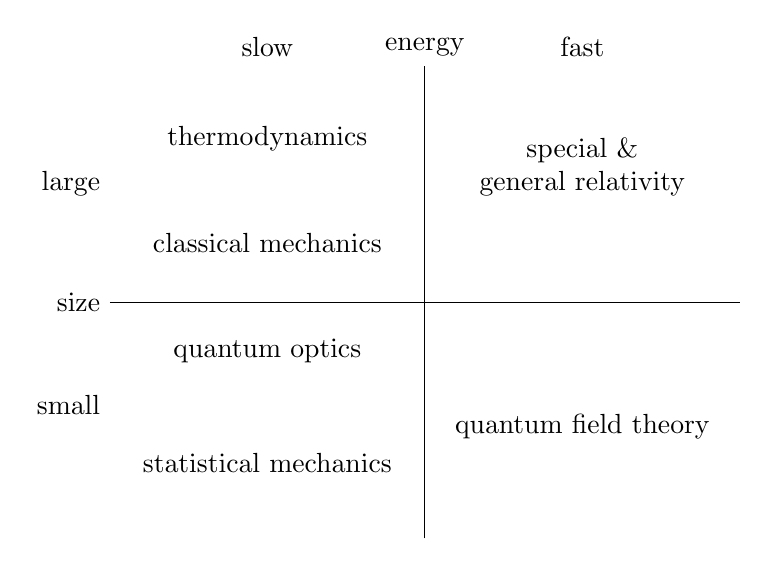
\begin{tikzpicture}
        \draw (-4,0) node[anchor=east] {size} -- (4,0);
        \draw (0,-3) -- (0,3) node[anchor=south] {energy};
        \draw[white] (-2.1,3) -- (-1.9,3) node[black,midway,anchor=south] {slow};
        \draw[white] (1.9,3) -- (2.1,3) node[black,midway,anchor=south] {fast};
        \draw[white] (-4,1.5) node[black,anchor=east] {large} -- (-3.9,1.5);
        \draw[white] (-4,-1.3) node[black,anchor=east] {small} -- (-3.9,-1.3);
        \draw[white] (-2.1,-0.35) -- (-1.9,-0.35) node[black,midway,anchor=north,align=center] {quantum optics};
        \draw[white] (-2.1,-1.8) -- (-1.9,-1.8) node[black,midway,anchor=north,align=center] {statistical mechanics};
        \draw[white] (-2.1,1.8) -- (-1.9,1.8) node[black,midway,anchor=south,align=center] {thermodynamics};
        \draw[white] (1.9,2.2) -- (2.1,2.2) node[black,midway,anchor=north,align=center] {\shortstack{special \&\\general relativity}};
        \draw[white] (1.9,-1.3) -- (2.1,-1.3) node[black,midway,anchor=north,align=center] {quantum field theory};
        \draw[white] (-2.1,0.5) -- (-1.9,0.5) node[black,midway,anchor=south,align=center] {classical mechanics};
    \end{tikzpicture}
\end{figure}

\textbf{Ingredients:}
\begin{itemize}
    \item harmonic oscillators
    \item Gaussian integrals
    \item Hamiltonian mechanics (canonical variables q and p)
    \item maths of operators - adjoint, self-adjoint, Hermitian, commutation relations
    \item QM in both Schrodinger and Heisenberg pictures
    \item density matrices
    \item classical EM - Maxwell's equations in Coulomb gauge - especially plane waves and dipoles
\end{itemize}

Hanbury Brown and Tiss:
\begin{equation}
    G(\tau) = I_A(t)I_B(t+\tau)
\end{equation}

\chapter{}
\section{Learning Outcomes}
To be able to state, explain and apply the operator formalism of the quantum harmonic oscillator to stuff

\section{Quantum Harmonic Oscillator}
\begin{align}
    F &= ma = m\ddot{x} \\
      &= -kx \\
    x(t) &= x_0\sin\om t \\
    p_x(t) &= p_0\cos\om t \\
    V(x) &= \frac12 kx^2 = \frac12 m\om^2x^2 \\
    \frac{\hbar^2}{2m}\frac{d^2\psi}{dx^2} &+ V(x)\psi(x) = E\psi \\
    E_n &= \left(n+\frac12\right)\hbar\om
\end{align}
   
\begin{figure}[H]
    \centering
    \begin{tikzpicture}
        \draw[->,thick] (-3,0) -- (3,0) node[anchor=south] {$x$};
        \draw[->,thick] (0,-0.3) -- (0,2) node[anchor=south] {$V(x)$};
        \draw (0,0) parabola (2.5,1.8);
        \draw (0,0) parabola (-2.5,1.8);
    \end{tikzpicture}
\end{figure}
Start with writing the Hamiltonian, then turn everything into operators
\begin{align}
    H &= \frac{p^2}{2m} + \underbrace{\frac12 m\om^2x^2}_{V(x)} \\
    p &\to \hp = -i\hbar\frac{d}{dx},~ x \to \hx \\
    [\hx,\hp] &= i\hbar \\
    H &= \frac{\hp^2}{2m} + \frac12m\om^2\hx^2 \\
    \ha &= \frac{1}{\sqrt{2m\hbar\om}}\left(m\om\hx+i\hp\right) \\
    \hag &= \frac{1}{\sqrt{2m\hbar\om}} \left(m\om\hx - i\hp\right) \\
    \hx &= \left(\frac{\hbar}{2m\om}\right)^{1/2}(\ha+\hag) \\
    \hp &= -i\left(\frac{m\hbar\om}{2}\right)^{1/2}(\ha-\hag) \\
    [\ha,\hag] &= \ha\hag - \hag\ha = 1 \\
    \hh &= \hbar\om(\hag\ha+\frac12) \\
    \hag\ha &= \hn,~ \hn|n\rangle = n|n\rangle \\
    \hh|n\rangle &= \hbar\om\left(n+\frac12\right)|n\rangle = E_n|n\rangle
\end{align}
How do the annihilation and creation operators, $\ha$ and $\hag$ interact with the number states, $|n\rangle$?
\begin{align}
    \hag|n\rangle &= \sqrt{n+1}|n+1\rangle \\
    \ha|n\rangle &= \sqrt|n-1\rangle
\end{align}
Together, the creation and annihilation operators are known as the \textit{ladder operators.}
Ladder operators move the system up or down the energy levels of the harmonic potential.
\begin{figure}[H]
    \centering
    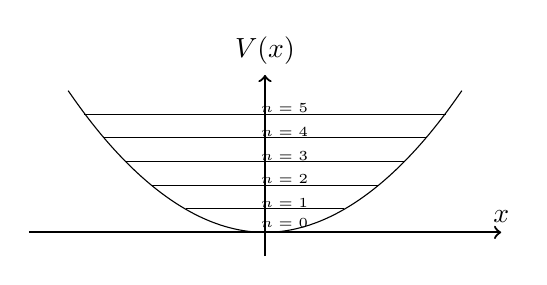
\begin{tikzpicture}
        \draw[->,thick] (-3,0) -- (3,0) node[anchor=south] {$x$} node[anchor=south,midway,xshift=7pt,yshift=-2pt] {\tiny $n=0$};
        \draw[->,thick] (0,-0.3) -- (0,2) node[anchor=south] {$V(x)$};
        \draw (0,0) parabola (2.5,1.8);
        \draw (0,0) parabola (-2.5,1.8);
        \draw (-2.3,1.5) -- (2.3,1.5) node[anchor=south,midway,xshift=7pt,yshift=-3pt] {\tiny $n=5$};
        \draw (-2.05,1.2) -- (2.05,1.2) node[anchor=south,midway,xshift=7pt,yshift=-3pt] {\tiny $n=4$};
        \draw (-1.78,0.9) -- (1.78,0.9) node[anchor=south,midway,xshift=7pt,yshift=-3pt] {\tiny $n=3$};
        \draw (-1.45,0.6) -- (1.45,0.6) node[anchor=south,midway,xshift=7pt,yshift=-3pt] {\tiny $n=2$};
        \draw (-1,0.3) -- (1,0.3) node[anchor=south,midway,xshift=7pt,yshift=-3pt] {\tiny $n=1$};
    \end{tikzpicture}
\end{figure}
We now have a partly new mathematical representation. 
Notice that the potential still remains positive, it does not go negative.
Therefore we must have:
\begin{align}
    \ha|0\rangle &= 0, \\
    \hn &= \hag\ha|0\rangle = 0. \\
    \implies \hh|0\rangle &= E_0|0\rangle = \frac12\hbar\om|0\rangle
\end{align}
So the ground state is labelled '0' but does not have $E=0$.\\
Now we introduce $\hog$ as the adjoint of $\ho$ if
\begin{align}
    \langle\psi|\ho|\phi\rangle &= \langle\phi|\hog|\psi\rangle^*\; \forall \psi,\phi
\end{align}
A self-adjoint operator is equivalent to a Hermitian operator, i.e. $\hn, \hh$.\\
For adjoint operators:
\begin{align}
    (\hat{A}+\hat{B})^\dagger &= \hat{A}^\dagger + \hat{B}^\dagger \\
    (\hat{A}\hat{B})^\dagger &= \hat{B}^\dagger\hat{A}^\dagger \\
    (c\hat{A})^\dagger &+ c^*\hat{A}^\dagger \\
    (\hat{A}^\dagger)^\dagger &= \hat{A}
\end{align}
More on the number states:
\begin{itemize}
    \item they are orthogonal
        \begin{align}
            \langle n|n\rangle &= 1 \\
            \langle n|m\rangle &= 0,~ n\neq m \\
            \langle n|m\rangle &= \delta_{n,m} \\
        \end{align}
    \item they form a basis (note: not mathematically a Hilbert space, but a Banah(?) space)
        \begin{align}
            |\psi\rangle &= \sum_n c_n|n\rangle \\
            0 &\leq n \leq \infty
        \end{align}
\end{itemize}

\section{Two Oscillators - independent}
\begin{align}
    |\psi_0\rangle &= \sum_n c_n|n\rangle_0 \\
    |\psi_1\rangle &= \sum_m c_m|m\rangle_1 \\
    |\psi_{01}\rangle &= \sum_{n,m} c_{n,m}|n\rangle_0|m\rangle_1
\end{align}
What we are doing is "tensoring" the Hilbert spaces: $\mathcal{H}_0 \otimes \mathcal{H}_1$:
\begin{align}
    |n\rangle_0|m\rangle_1 &\equiv |n\rangle_0\otimes|m\rangle_1.
\end{align}
Now we have the operators, $\ha_0,\hag_0,\ha_1,\hag_1$:
\begin{align}
    \ha_0 \otimes \mathbb{I}_1&,~ \mathbb{I}_0\otimes \ha_1,\dots \\
    [\ha_0,\ha_1] &= [\ha_0,\hag_1] = 0 \\
    \hh &= \hh_0\otimes\mathbb{I}_1 + \mathbb{I}_1\otimes\hh_1 
\end{align}
Note this is for non-interacting oscillators. 
For interacting, 
\begin{align}
    \hh &= \hh_0\otimes\mathbb{I}_1 + \mathbb{I}_1\otimes\hh_1 + \mathcal{H}_{int}.
\end{align}

\chapter{}
\section{Learning Outcomes}
To be familiar with the route to quantisation of the electromagnetic field, in particular to:
\begin{itemize}
    \item Explain and state the description of the electromagnetic field in terms of modes, including polarization
    \item Be familiar with the equivalence between a mode of the field and a quantum harmonic oscillator
    \item To explain the form of (but not derive) expressions for the Hamiltonian of the electromagnetic field, and the electric and magnetic fields in terms of the creation and annihilation operatoes
    \item To recognise and explain the concepts of the Schrodinger and Heisenberg representations, and to explain which is being applied
    \item To explain and apply the concepts of adjoint and self-adjoint operators and their matrix elements
\end{itemize}

\section{Quantising the EM field}
Consider an EM scalar potential, $\phi=0$ (no free charges), and a vector potential, $\unl{A}$.
\begin{align}
    \E(\vr,t) &= \frac{\p}{\p t}\unl{A} & \B(\vr,t) &= \del\times\unl{A}(\vr,t) \\
    \grad\left[\grad\cdot\unl{A}\right] &- \del^2\unl{A} + \frac{1}{c^2}\frac{\p^2}{\p t^2}\unl{A} = 0
\end{align}
Coulomb gauge, $\del\cdot\unl{A} = 0$.
\begin{align}
    \unl{A} &= \sum_{\unl{k}} \left\{ \unl{A}_{\unl{k}}\exp\left[i(\unl{k}\cdot\unl{r}-\om_kt)\right] + \unl{A}^*_{\unl{k}}\exp\left[-i(\unl{k}\cdot\unl{r} - \om_kt)\right]\right\} \\
    \om_k &= c|k|,~ \unl{k}\cdot\unl{A}_{k} = 0
\end{align}
Polarisation vectors, $\ve_{k1},\ve_{k2}$ - orthonormal vectors perpendicular to $\unl{k}$.
\begin{align}
    \unl{A}_k &= A_{k1}\ve_{k1} + A_{k2}\ve_{k2} \\
    \unl{A} &= \sum_{\unl{k},s} A_{\unl{k},s}\ve_{\unl{k},s}\exp\left\{i(\unl{k}\cdot\vr-\om_kt)\right\} + A_{\unl{k},s}^*\ve_{\unl{k},s}\exp\left\{-i(\unl{k}\cdot\vr-\om_kt)\right\}
\end{align}
The labels of the modes are $\unl{k},s$, $s\in1,2$. 
They gives us the: direction; wavelength, $\frac{2\pi}{|\unl{k}|}$; and polarisation, $s$.\\
To quantise this classically:
\begin{align}
    H &= \frac12\e_0 \int \left(\E\cdot\E + c^2\B\cdot\B\right)\,dV \\
      &= 2\e_0 V \sum_{\unl{k},s} \om_k^2 A_{\unl{k},s}A_{\unl{k},s}^* \\
    A_{\unl{k},s} &= \frac{1}{2\om_k\sqrt{\e_0V}} \left\{\om_kq_{\unl{k},s} + ip_{\unl{k},s}\right\} \\
    A_{\unl{k},s}^* &= \frac{1}{2\om_k\sqrt{\e_0V}} \left\{\om_kq_{\unl{k},s} - ip_{\unl{k},s}\right\}
\end{align}
$q_{\unl{k},s},p_{\unl{k},s}$ canonical coordinates $(x,p)$.
\begin{align}
    H_{\unl{k},s} &= \frac12\left(p^2_{\unl{k},s} + \om_k^2q_{\unl{k},s}\right)
\end{align}
Harmonic oscillator $m=1$, $x\leftrightarrow p$.
To transfer this from classical to quantum, you simply convert everything to its operator form. 
For a single mode:
\begin{align}
    \hh_{\unl{k},s} &= \left(\hag_{\unl{k},s}\ha_{\unl{k},s} + \frac12\right)\hbar\om_k \\
    [\ha_{\unl{k},s},\hag_{\unl{k},s}] &= 1 \\
    \hag_{\unl{k},s}\ha_{\unl{k},s} &= \hn_{\unl{k},s}
\end{align}
Now we have eigenstates, $|n\rangle_{\unl{k},s}$.
Note: modes are not always equal to photons, but you can have photons spread over several modes. \\
Going back on the substitution:
\begin{align}
    \hat{A}_{\unl{k},s} &= \sqrt{\frac{\hbar}{2\om_k\e_0V}}\ha_{\unl{k},s} & \hat{A}_{\unl{k},s}^\dagger &= \sqrt{\frac{\hbar}{2\om_k\e_0V}}\hag_{\unl{k},s}
\end{align}
From these, we can find the quantised electric and magnetic field expressions. 
We will mostly be concerned with the electric field throughout this course as it has a much stronger interaction with matter than the magnetic. 
\begin{align}
    \hat{\E}_{\unl{k},s}(\vr,t) &= i\left(\frac{\hbar\om_k}{2\e_0V}\right)^{1/2}\ve_{\unl{k},s}\left[\ha_{\unl{k},s}\exp\{i(\unl{k}\cdot\vr-\om_kt)\} - \hag_{\unl{k},s}\exp\{-i(\unl{k}\cdot\vr-\om_kt)\}\right]
\end{align}

\section{Multimode Fields}
\begin{align}
    \hat{H}_{\unl{k},s} &= \sum_{\unl{k},s} \hbar\om_k \left(\hag_{\unl{k},s}\ha_{\unl{k},s} + \frac12\right)
\end{align}
So the modes are independent of each other, but will interact through matter. 
We have a basis of 
\begin{equation}
    |n_1n_2n_3\dots\rangle \equiv |n_1\rangle_{\unl{k}1,s}\otimes|n_2\rangle_{\unl{k}2,s}\otimes\dots
\end{equation}
Now we can write the electric field operator:
\begin{align}
    \hat{\E}(\vr,t) &= \sum_{\unl{k},s} \hat{\E}_{\unl{k},s}(\vr,t) \\
                    &= \sum_{\unl{k},s} i\left(\frac{\hbar\om_k}{2\e_0V}\right)^{1/2}\ve_{\unl{k},s}\left\{\ha_{\unl{k},s}\exp[i(\unl{k}\cdot\vr-\om_kt)] + \hag_{\unl{k},s}\exp[-i(\unl{k}\cdot\vr-\om_kt)]\right\}
\end{align}
This is written in the Heisenberg representation. 
Now if we look at the expectation value, for one mode of the electric field
\begin{align}
    {}_{\unl{k},s}\langle n|\hat{\E}(\vr,t)|n'\rangle_{\unl{k},s}
\end{align}
This is time dependent as seen by the field operator and will oscillate in time through some means. 
As a reminder, consider an operator in the Heisenberg picture:
\begin{align}
    \hat{O}_H(t) &= \hat{U}^\dagger(t,t_0)\hat{O}\hat{U}(t,t_0) \\ 
    \hat{U}(t,t_0) &= \exp
\end{align}










\textit{LOs for L2}
\end{document}


















